\documentclass[pdftex,12pt,a4paper]{article}

\usepackage{graphicx}  
\usepackage[margin=2.5cm]{geometry}
\usepackage{breakcites}
\usepackage{indentfirst}
\usepackage{pgfgantt}
\usepackage{pdflscape}
\usepackage{float}
\usepackage{epsfig}
\usepackage{epstopdf}
\usepackage[cmex10]{amsmath}
\usepackage{stfloats}
\usepackage{multirow}

\renewcommand{\refname}{REFERENCES}
\linespread{1.3}

% REQUIRED FOR INSETYING SOME SHITASS ASSEMBLY CODE INTO TO LATEX BIATCH fuck this retarded thing, science my ass
\usepackage{listings}
\usepackage{xcolor}
\definecolor{codegreen}{rgb}{0,0.6,0}
\definecolor{codegray}{rgb}{0.5,0.5,0.5}
\definecolor{codepurple}{rgb}{0.58,0,0.82}
\definecolor{backcolthe}{rgb}{0.95,0.95,0.92}
\definecolor{CommentGreen}{rgb}{0,.6,0}
% bu salak seyin son satiri bosluk olunca calismiyor kendimi sikcem simdi
% Icine comment de konmuyor

\lstset{
    numbers=left,
    basicstyle=\small\ttfamily,
    numberstyle=\tiny,
    keywordstyle=\color{blue}\bfseries,
    keywordsprefix=B,
    language={[x86masm]Assembler},
    breaklines=true,
    commentstyle=\color{codegreen},
    keywordstyle=\color{blue},
    keywordstyle=[2]\color{orange},
    keywordstyle=[3]\color{codegray},
    numberstyle=\tiny\color{codegray},
    stringstyle=\color{codepurple},
    showtabs=false,
    frame=single,
    keepspaces,
    escapechar=@,
}



\usepackage{mathtools}
%\newcommand{\HRule}{\rule{\linewidth}{0.5mm}}
\thispagestyle{empty}
\begin{document}
\begin{titlepage}
\begin{center}
\textbf{}\\
\textbf{\Large{ISTANBUL TECHNICAL UNIVERSITY}}\\
\vspace{0.5cm}
\textbf{\Large{COMPUTER ENGINEERING DEPARTMENT}}\\
\vspace{2cm}
\textbf{\Large{BLG 351E\\ MICROCOMPUTER LABORATORY\\ EXPERIMENT REPORT}}\\
\vspace{2.8cm}
\begin{table}[ht]
\centering
\Large{
\begin{tabular}{lcl}
\textbf{EXPERIMENT NO}  & : & 3 \\
\textbf{EXPERIMENT DATE}  & : & 16.10.2019 \\
\textbf{LAB SESSION}  & : & WEDNESDAY - 13.30 \\
\textbf{GROUP NO}  & : & G10 \\
\end{tabular}}
\end{table}
\vspace{1cm}
\textbf{\Large{GROUP MEMBERS:}}\\
\begin{table}[ht]
\centering
\Large{
\begin{tabular}{rcl}
150170062  & : & Mehmet Fatih YILDIRIM \\
150180704  & : & Cihat AKK\.{I}RAZ \\
150180705  & : & Batuhan Faik DER\.{I}NBAY \\
150180707  & : & Fatih ALTINPINAR \\
\end{tabular}}
\end{table}
\vspace{2.8cm}
\textbf{\Large{FALL 2019-2020}}

\end{center}

\end{titlepage}


\thispagestyle{empty}
\addtocontents{toc}{\contentsline {section}{\numberline {}FRONT COVER}{}}
\addtocontents{toc}{\contentsline {section}{\numberline {}CONTENTS}{}}
\setcounter{tocdepth}{4}
\tableofcontents
\clearpage

\setcounter{page}{1}

\section{INTRODUCTION}
\paragraph{}
In this experiment, with the purpose of getting more familiar with assembly language and understanding what happens in computer's low level when we write programs some mathematical algorithms are coded using MSP430 microcontroller. Then these mathematical algorithms will be used as functions to obtain more functionality from the written assembly program.

\section{MATERIALS AND METHODS}

This experiment is completed by using a MSP430G2553 microprocessor. This microprocessor is programmed by using Code Composer Studio for the desired tasks on the experiment handout. During coding several sources have been used:

\begin{itemize}
    \item MSP430 Education Board Manual \cite{ref2}
    \item MSP430 Architecture Chapter 4 \cite{ref3}
    \item MSP430 Instruction Set \cite{ref4}
\end{itemize}

\subsection{Part 1}
In the first part of the experiment, the microprocessor was programmed to perform some steps from Russian Peasant Division for modulus operation.

\newline
In order to implement the given task, team created following piece of code given in Figure \ref{code:part1}

\begin{figure}[H]
    \centering
    \begin{lstlisting}[language={[x86masm]Assembler}]
; R10 = A, R11 = B, R12 = C, R13 = D
initial		mov	#151, R10
		mov	#8, R11

main		mov	R11, R12
		mov	R10, R13
		mov	R10, R9
		rra	R9

cLEthan		cmp	R12, R9
		jge	multiply
		jmp	bLEthan

multiply	rla	R12
		jmp	cLEthan

bLEthan		cmp	R11, R13
		jge	subtract
		jmp	exit

subtract	cmp	R12, R13
		jl	divide
		sub	R12, R13
		jmp	divide

divide		rra	R12
		jmp	bLEthan

exit		jmp	exit
    \end{lstlisting}
    \label{code:part1}
    \caption{Assembly Code of Part 1}
\end{figure}

 For better understanding, the code can be further examined line by line as seen below:
\begin{itemize}
    \item Line 1: Explains as a comment which register is used for which variable.
    \item Line 2-3: Initial values of the variables A and B are assigned.
    \item Line 5-6: The values of A and B are given to D and C, respectively, as asked in the experiment booklet.
    \item Line 7-8: In line 7, an additional variable (register) which will keep halved value of A is given its initial value, i.e. A. In line 8, its value is halved so that it keeps the half of the value of A, obviously.
    \item Line 10-12: In line 10, the value of C is compared with A/2. In line 11, if A/2 is greater than or equal to C, it jumps to multiply. If not, in line 12, it jumps to bLEthan.
    \item Line 14-15: In line 14, C is multiplied by 2 as asked in the experiment booklet. In line 15, it jumps right back to cLEthan to implement the loop which will end when C is greater than A/2.
    \item Line 17-19: In line 17, B is compared with D. In line 18, if D is greater than or equal to B, it jumps to subtract. If not, in line 19, it jumps to exit because if this loop ends, there will be nothing left to do.
    \item Line 21-24: In line 21, C is compared with D. In line 22, if D is less than C, it jumps directly to divide. If not, in line 23, the value of C is subtracted from D and then in line 24, it jumps to divide eventually.
    \item Line 26-27: In line 26, the value of C is halved as asked. In line 27, it jumps to bLEthan to construct the loop which iterates through until B gets larger than D.
    \item Line 29: The program enters an infinite exit loop for debugging purposes.
\end{itemize}

\subsection{Part 2}
Second part of the experiment demands such an implementation which will find first 50 prime numbers by using the code in Part 1 like a function.
\begin{figure}[H]
    \centering
    \begin{lstlisting}[language={[x86masm]Assembler}]
; R10 = A, R11 = B, R12 = C, R13 = D, R4 = addr_primes, R5 = prime_index, R6 = prime_test, R7 = iteration, R8 = temp_modulus    
		mov		#primes, R4
		mov		#primes, R5
		mov		#2, R6
		mov		#2, R7

main		cmp		#0, 98(R4)
		jne		exit
		mov		R6, R10
		mov		R7, R11
		jmp		modulus

append		cmp		#0 ,R13
		jne		addition
		cmp		R6, R7
		jeq		add_prime
		inc		R6
		mov		#2, R7
		jmp		main

addition	inc		R7
		mov		R7,	R11
		jmp		modulus

add_prime       mov		R6, 0(R5)
		add		#2, R5
		inc		R6
		mov		#2, R7
		jmp		main

modulus		mov		R11, R12
		mov		R10, R13
		mov             R10, R8
		rra		R8

cLEthan		cmp		R12, R8
		jge		multiply
		jmp		bLEthan\end{lstlisting}
    \label{code:part2_1}
    \caption{Assembly Code 1$^{st}$ Snippet of Part 2}
\end{figure}
\begin{figure}[H]
    \centering
    \begin{lstlisting}[language={[x86masm]Assembler}, firstnumber=39]
multiply	rla		R12
		jmp		cLEthan

bLEthan		cmp 	        R11, R13
		jge		subtract
		jmp		append

subtract	cmp		R12, R13
		jl		divide
		sub		R12, R13
		jmp		divide

divide		rra		R12
		jmp		bLEthan

exit		jmp		exit

		.data
primes		.space	100
    \end{lstlisting}
    \label{code:part2_2}
    \caption{Assembly Code 2$^{nd}$ Snippet of Part 2}
\end{figure}

For better understanding, further examination of the code, line by line if necessary, is required:

\begin{itemize}
    \item Line 30-53: These lines are copied from Part 1. Only difference is in line 19 in Figure \ref{code:part1} is replaced with line 44 in Figure \ref{code:part2_2}.
    \item Line 2-3: Start address of primes array is stored in both $R4$ and $R5$. $R5$ indicates index of the next prime number that will be written on the array. $R4$ will be used for termination after finding 50 prime numbers.
    \item Line 4-5: R6 holds the number that is tested if it is prime or not. $R7$ holds the number that R6 is going to be divided in order to understand prime status of $R6$. The number range starts from 2 and increases until the value that is in $R6$.
    \item Line 7-8: Since program will find first 50 prime numbers, code will loop until R5 hits end of the primes array.
    \item Line 9-11: Modulus function is called and it will calculate $R10 \mod R11$ and return value by $R13$. \item Line 13-14: If return value from modulus which is remainder, is not zero jump to $addition$ label in Line 21. Since it means the value in $R6$ cant be divided to $R7$ without a remainder.
    \item Line 15-16: If remainder is zero, Equality of $R6$ and $R7$ is checked. If they are it means value in $R6$ can only be divided by itself without a remainder. Thus it is a prime and has to be added to the primes array. Line 16 jumps to $add_prime$ label in Line 25.
    \item Line 17-18: If remainder is zero but $R6$ is not equal to $R7$. It means the value in $R6$ can be divided by something that is not itself. This indicates the value in $R6$ is not a prime number thus testing of next number can begin. This is sustained by incrementing $R6$ and setting $R7$ back to $2$ then jumping to main label in Line 7.
    \item Line 21-23: If $R6$ cannot be divided to $R7$ and $R6$ is not equal to $R7$, $R7$ should be incremented by one in order to test $R6$ by the next number.
    \item Line 25-26: If $R6$ contains a prime, it is added to the place in the memory which is pointed by address value in $R5$. Then $R5$ is incremented by 2 for writing following prime number into next index.
    \item Line 27-29: In order to check next number is prime or not $R6$ is incremented by one and $R7$ is set back to 2. Program jumps back to main label in order to test next value in $R6$.
    
\end{itemize}

\subsection{Part 3}
\newline
In this part the team is asked to implement Goldbach's Conjecture for even integers between $[200-298]$ and save corresponding values to the memory using the MSP430. As mentioned in Part 2, first 50 prime number are found and appended to the "primes" array (See Figure \ref{code:part3_1}-\ref{code:part3_2}).
\begin{itemize}
    \item Line 1-54: The part of code that is responsible for finding the prime numbers and storing them in the "primes" array.
    \item Line 9: Notice that after appending appropriate prime numbers to "primes" array, the program jumps unconditionally to the "part3" section of the code where the Goldbach's Conjecture is implemented.
\end{itemize}
\newline
In the upcoming part of the code the team decided to use the following approach given in C-like pseudo-code (See Figure \ref{code:part3_C}). Refer to given pseudo-code as felt necessary.
For better understanding of the Goldbach's Conjecture the code, Figures \ref{code:part3_1}-\ref{code:part3_3}, can be analyzed as follows:
\begin{itemize}
    \item Line 56: Commented line. Gives the reader a great insight of what the registers will be storing during the program. Further explaining, "i", "j", and "k" variables are indexes for three nested while loops. "R7" holds the end memory address of "primes" array. "R8" and "R9" hold the addresses of memory locations in the "primes" array and are uses as pointers for variables "j" and "k".
    \item Line 58-63: Initial values of "i", "R7", "R8" and "R9" are stored.
    \item Line 64,66: Values of "j" and "k" reset respectively since end of the while loop reached.
    \item Line 67-70: Prime numbers pointed by "j" and "k" are added up and compared for equality. (Lines 5-7 in Figure \ref{code:part3_C})
    \item Line 71-74: Checks whether "k" reached to the end of "primes" array. If so jumps back to the respective while loop, if not increments "k" by two (since the data stored are 2 bytes) and repeats itself.
    \item Line 76-79: Checks whether "j" reached to the end of "primes" array. If so jumps back to the respective while loop, if not increments "j" by two (since the data stored are 2 bytes) and repeats itself.
    \item Line 81-84: This label is called only when conjecture condition is satisfied. Stores the memory addresses of prime numbers -as directed in the laboratory instructions- in respective arrays.
    \item Line 86-89: Checks whether "i" reached to the end of even integers that are needed to be tested. If so exits the loop, hence the program, if not increments "i" by two (since the next even number needs to be checked) and repeats itself.
    \item Line 91: Infinite exit loop for debugging purposes.
    \item Line 94-96: Memory allocations for respective arrays. Notice that each array has a size of 100 bytes (50 words).
\end{itemize}

\newline
When the previously explained Goldbach's Conjecture algorithm executes successfully,  the array "primes" holds the first 50 prime integers. Meanwhile, the arrays "array1" and "array2" store the first prime integer tuples of that's sum equal to the even integer at the same index starting from 200 respectively.

\begin{figure}[H]
    \centering
\begin{lstlisting}[language={C}, numbers=left]
int i = 200; int* end_prime_addr = primes + 0x062; int** arr1_ptr = array1; int** arr2_ptr = array2;
while (i<300){  // Look through every even number between
    while (j<end_prime_addr){   // While j has values to test
        while (k<end_prime_addr){   // While k has values to test
                int tmp = &j;
                tmp += &k;
                if (i == tmp){  // If conjecture is found store its memory addr in memory
                    &arr1_ptr = j;
                    &arr2_ptr = k;
                    arr1_ptr += 0x02;
                    arr2_ptr += 0x02;
                }
            k+=0x02;
        }
        j+=0x02;
    }
i+=2;
}
\end{lstlisting}
    \caption{C-like Pseudo-code of Goldbach's Conjecture Algorithm}
    \label{code:part3_C}
\end{figure}

\begin{figure}[H]
    \centering
\begin{lstlisting}[language={[x86masm]Assembler}, numbers=left]
; R10 = A, R11 = B, R12 = C, R13 = D, R4 = addr_primes, R5 = prime_index, R6 = prime_test, R7 = iteration, R8 = temp_modulus

			mov		#primes, R4
			mov		#primes, R5
			mov		#2, R6
			mov		#2, R7
    
main	             	cmp		#0, 98(R4)
			jne		part3
			mov		R6, R10
			mov		R7, R11
			jmp		modulus

append	             	cmp		#0 ,R13
			jne		addition
			cmp		R6, R7
			jeq		add_prime
			inc		R6
			mov		#2, R7
			jmp		main

addition                inc		R7
			mov		R7,	R11
			jmp		modulus

add_prime               mov		R6, 0(R5)
			add		#2, R5
			inc		R6
			mov		#2, R7
			jmp		main

modulus	    	        mov		R11, R12
			mov		R10, R13
			mov 	        R10, R8

			rra		R8
cLEthan	    	        cmp		R12, R8
			jge		multiply
			jmp		bLEthan    \end{lstlisting}
    \caption{Assembly Code 1\textsuperscript{st} Snippet of Part 3}
    \label{code:part3_1}
\end{figure}

\begin{figure}[H]
    \centering
\begin{lstlisting}[language={[x86masm]Assembler}, numbers=left, firstnumber=41]
multiply    	        rla		R12
			jmp		cLEthan

bLEthan	    	        cmp 	        R11, R13
			jge		subtract
			jmp		append

subtract    	        cmp		R12, R13
			jl		divide
			sub		R12, R13
			jmp		divide

divide	    	        rra		R12
			jmp		bLEthan

; R4= i, R5= j, R6= k, R7= end_prime_addr, R8= arr1_ptr, R9= arr2_ptr, R10= tmp

part3	    	        mov 	        #200, R4
			mov		#primes, R7
			add		#98, R7
			mov		#array1, R8
			mov		#array2, R9

forI	    	        mov		#primes, R5

forJ	    	        mov		#primes, R6
forK	    	        mov		0(R5), R10
			add		0(R6), R10
			cmp		R4, R10
			jz		add_comp
			cmp		R7, R6
			jz		iterJ
			add		#2, R6
			jmp		forK

iterJ	    	        cmp		R5, R7
			jz		iterI
			add		#2, R5
			jmp 	        forJ\end{lstlisting}
    \caption{Assembly Code 2\textsuperscript{nd} Snippet of Part 3}
    \label{code:part3_2}
\end{figure}
			
\begin{figure}[H]
    \centering
\begin{lstlisting}[language={[x86masm]Assembler}, numbers=left, firstnumber=81]
add_comp    	        mov		R5, 0(R8)
			mov		R6, 0(R9)
			add		#2, R8
			add		#2, R9

iterI	    	        cmp		#300, R4
			jz		exit
			add		#2, R4
			jmp		forI

exit                    jmp		exit

			.data
primes		        .space	100
array1		        .space	100
array2		        .space	100
\end{lstlisting}
    \caption{Assembly Code 3\textsuperscript{rd} Snippet of Part 3}
    \label{code:part3_3}
\end{figure}

\section{RESULTS}
In the first part, modulus of any number can be taken with the written assembly code. If you give an example: Modulus of A(151) was calculated with coded program like given steps in Figure \ref{fig:modulus}:

\begin{figure}[H]
    \centering
    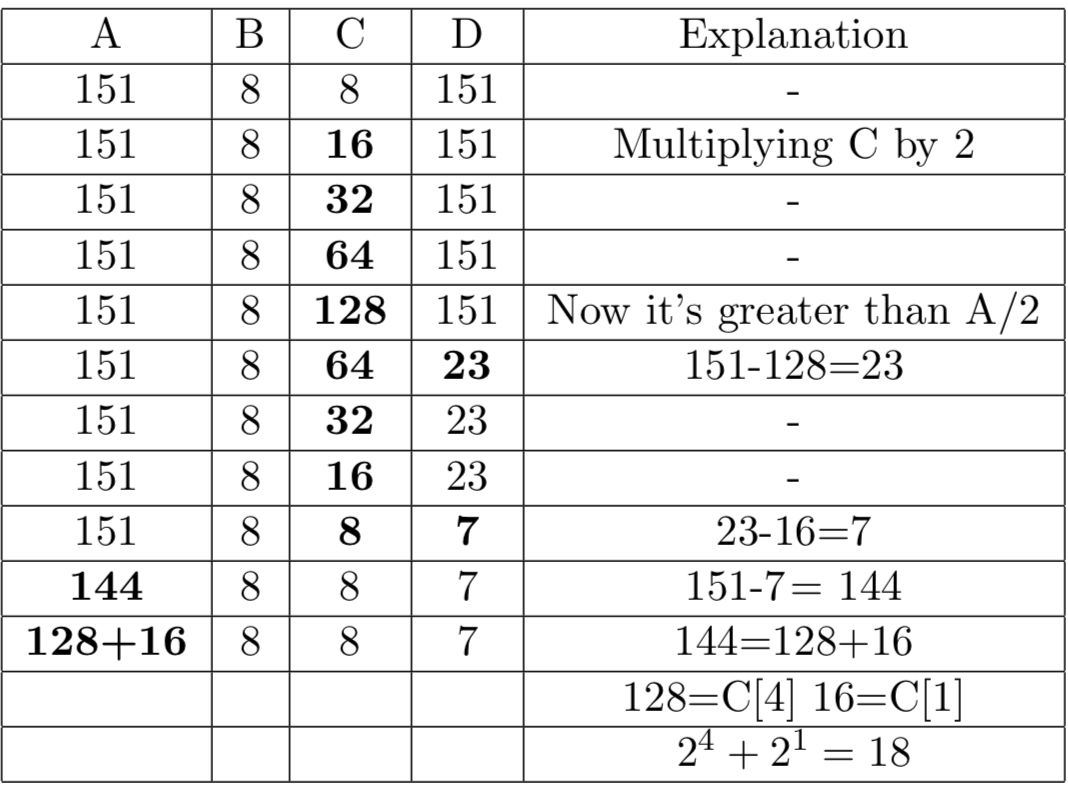
\includegraphics[width=0.75\textwidth]{modulus.png}
    \caption{Modulus steps while program execution}
    \label{fig:modulus}
\end{figure}

\paragraph{}
In the second part, the first 50 prime numbers were found and saved them to a memory address. Prime numbers were found using the code in the first part. With the memory browser in the Code Composer written values to memory are observed like in Figure \ref{fig:memory}.

\begin{figure}[H]
    \centering
    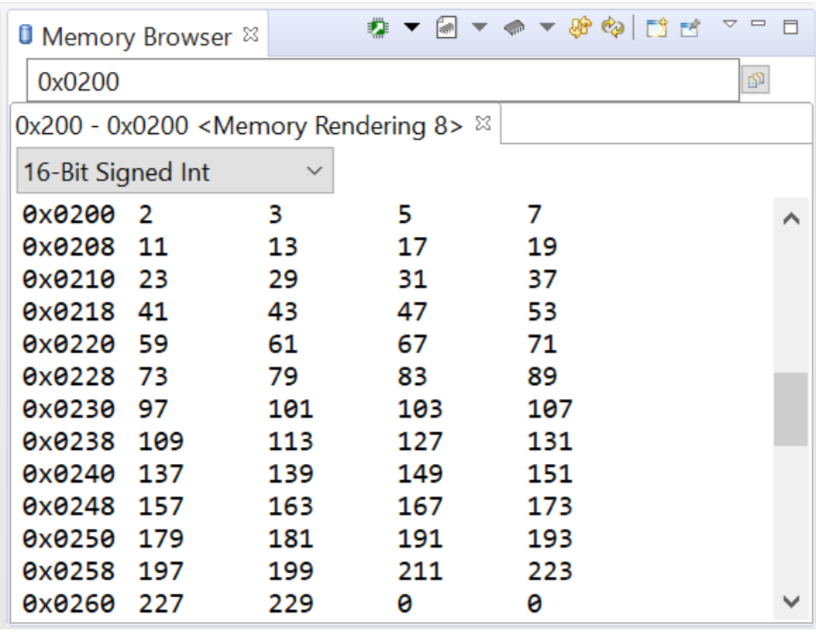
\includegraphics[width=0.75\textwidth]{memory.png}
    \caption{Observation of prime numbers written to memory}
    \label{fig:memory}
\end{figure}

\paragraph{}
The final part is widely explained in the methods section. Results of this part is observed using memory window in Code Composer. 

% abi bu challenge i kabul ediyor musun? xd

\section{DISCUSSION}
The first and second parts required us to think. Since first part will be used in following one, the code had to written as a function. This created several issues such as how to return result from function, how to pass parameters to function and so on. Team understood what is desired and implemented carefully given task. In the third part, it was learnt how nested loops are implemented in Assembly language. Our team coded first two parts before coming to the lab session. During lab session as debugging code some errors are fixed.

\newline
In the experiment, it was observed that with MSP430 microprocessor you can do memory to memory operation. This can be great benefit of MSP430 beside low power consumption.
\newline
Please refer to section 2 "MATERIALS AND METHODS" for exclusively detailed information, tables, images, analysis, interpretation and results, covering all the required material under other sections.
\section{CONCLUSION}
The team has learned assembly language more deeply and coded desired tasks successfully. The team finished the tasks as quickly as usual. At the end of the experiment, memory manipulation is understood better. Also, seeing how nested loops working in low level was a big gain for the team. Implementing the function in Part 1, gave team more experience about how function calls work on CPU level. While writing the code, team saw that, called function overrides current values in registers. Which creates a scope problem in the code. This will be resolved with the usage of stack, which is the topic of the next experiment.
\newline
In conclusion, the team got more experience with the MSP430 microcontroller and assembly language.



\nocite{overleaf}
\nocite{reportGuide}
\newpage
\addcontentsline{toc}{section}{\numberline {}REFERENCES}

\bibliographystyle{unsrt}
\bibliography{reference}

\end{document}

